%
% This is the epigraph file (epigraph.tex)
%
%\newpage\null\thispagestyle{empty}
%\begin{center}
%    \begin{figure*}
%        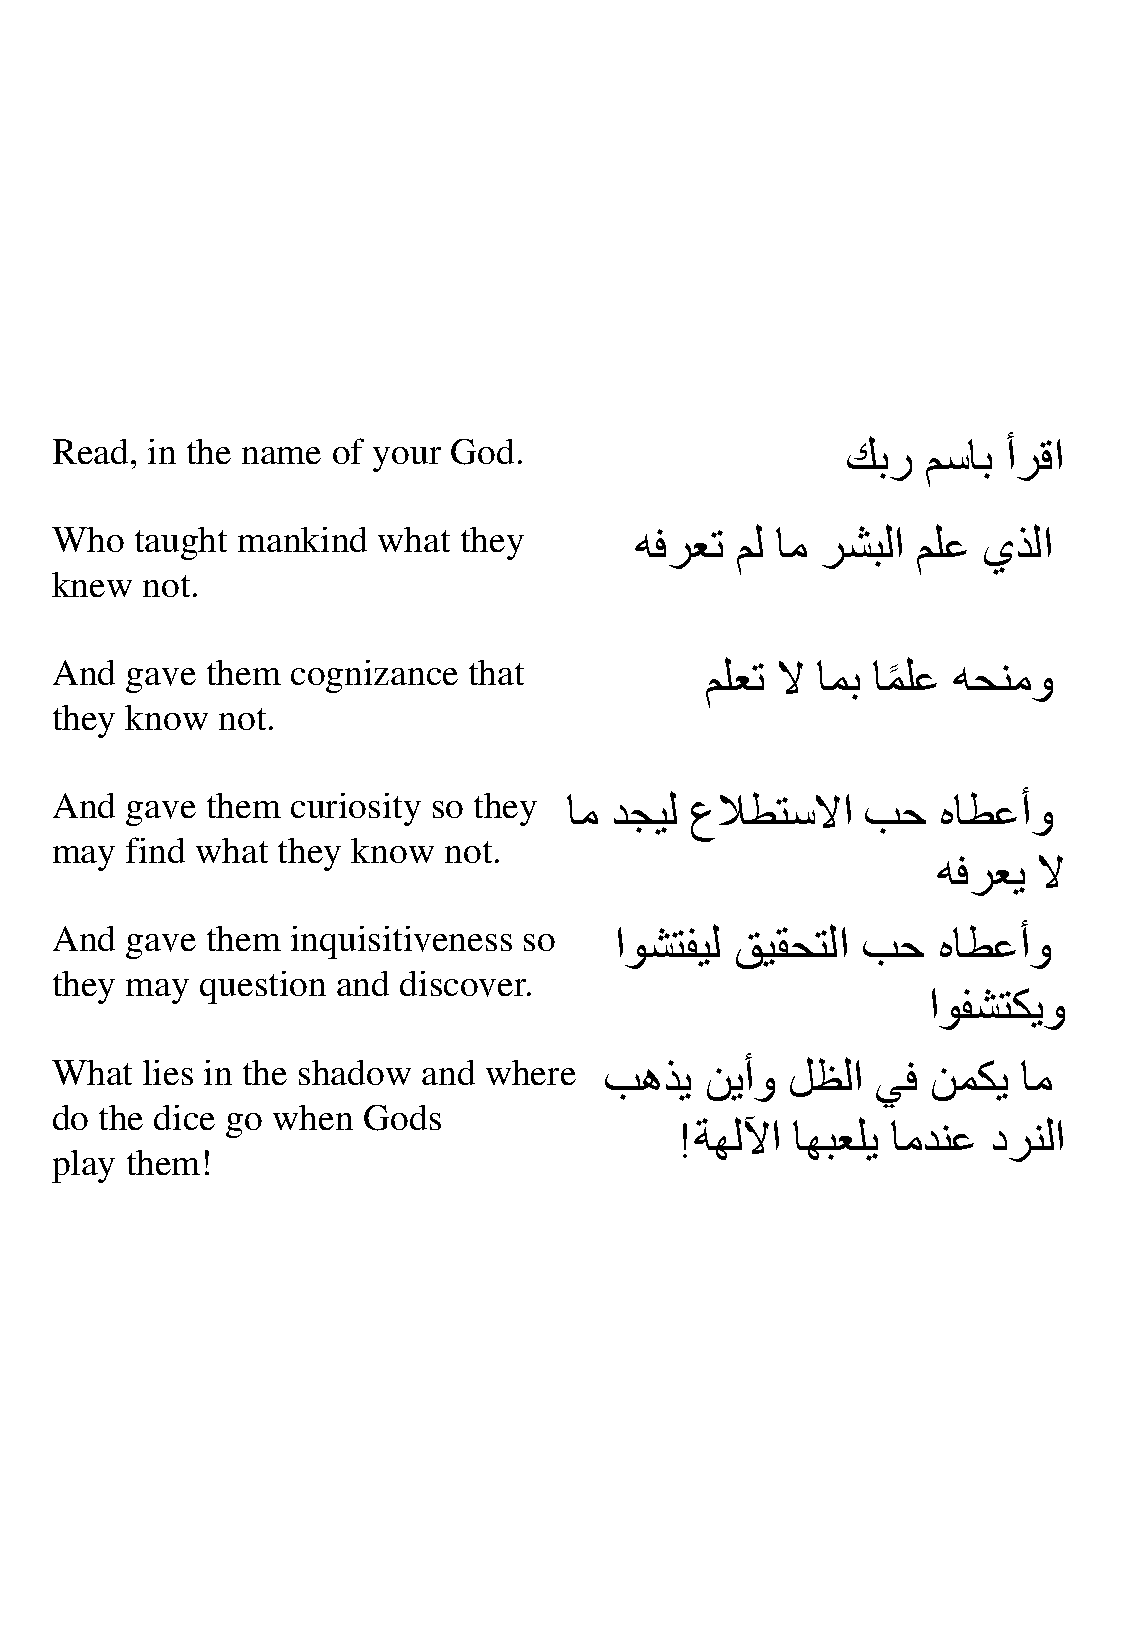
\includegraphics[width=1\textwidth]{figures/epigraph/thesis_epigraph_v2.pdf}
%        \captionsetup{labelformat=empty}
%        \caption[]{}
%    \end{figure*}
%\end{center}

\newpage\null\thispagestyle{empty}\newpage
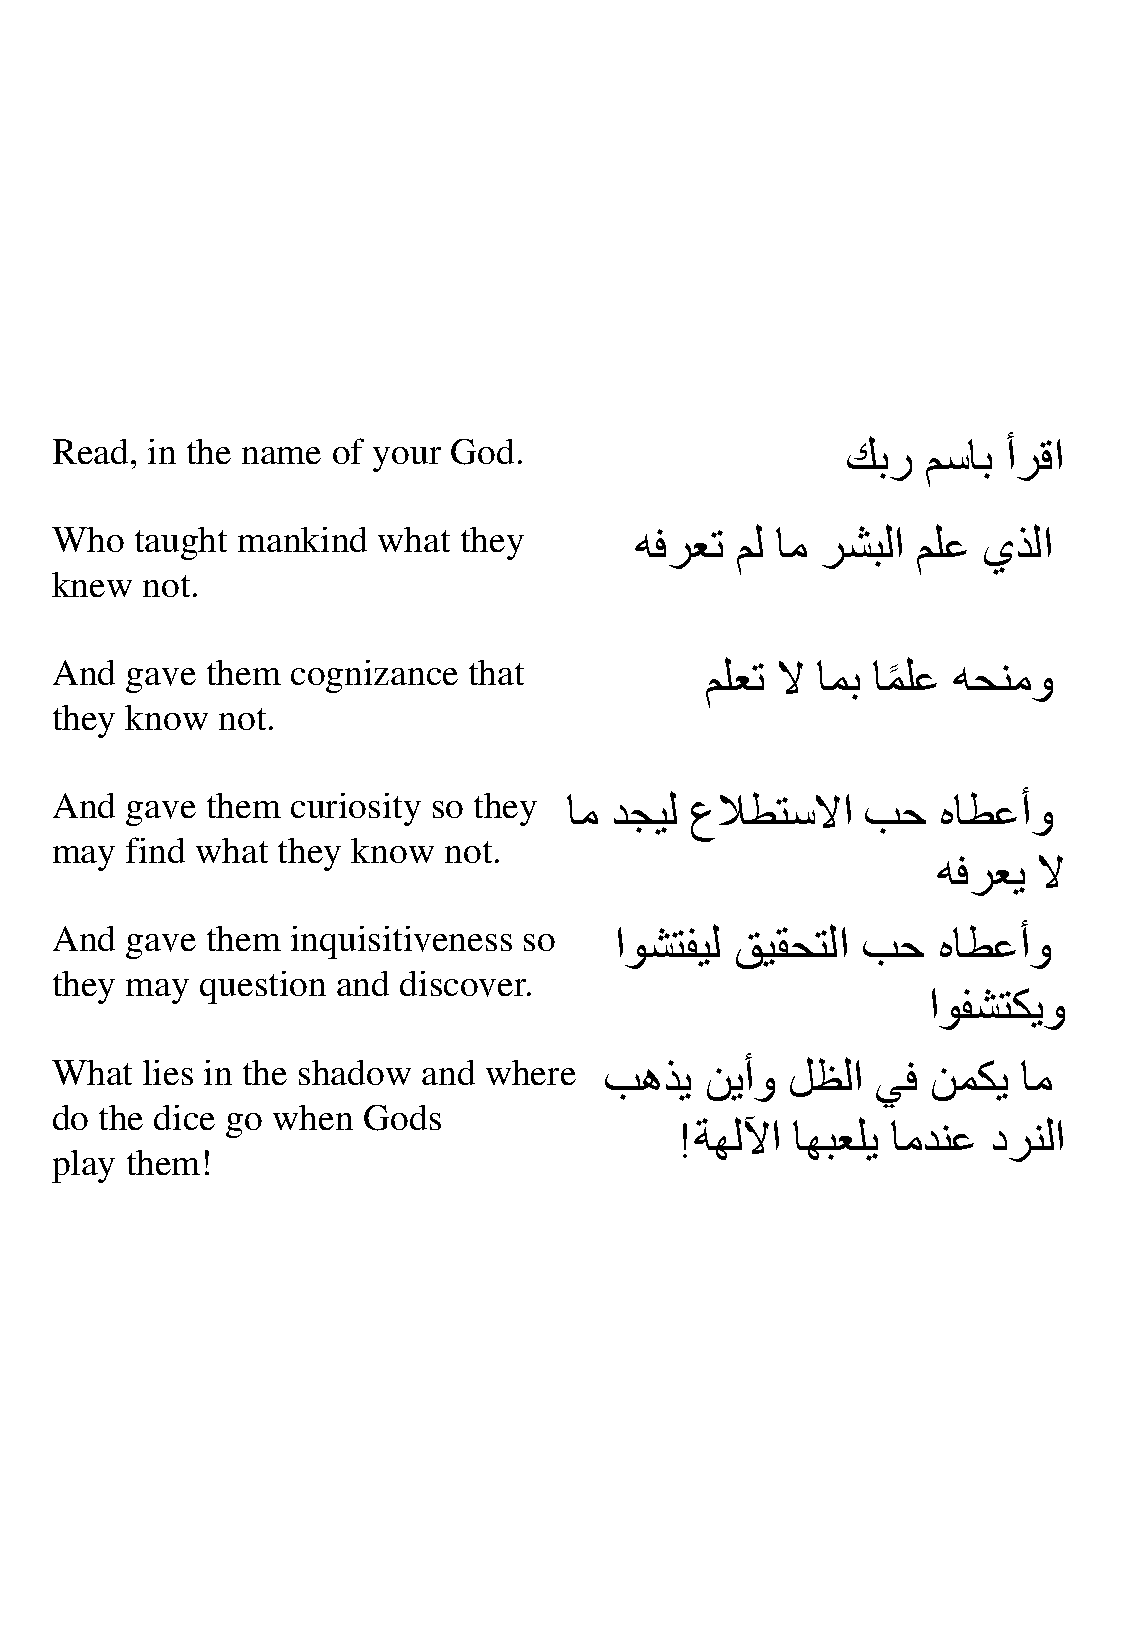
\includepdf{figures/epigraph/thesis_epigraph_v2.pdf}

\newpage\null\thispagestyle{empty}\newpage

\vspace*{\fill} \hspace{-3.2em}“This is a work of fiction. Still, given an infinite number of possible
worlds, it must be true on one of them. And if a story set in an infinite number of possible worlds
is true in one of them, then it must be true in all of them. So maybe, it's not as fictional as we
think.”\\
\hspace*{0pt}\hfill ― Neil Gaiman, InterWorld
\vspace*{\fill}

\newpage\null\thispagestyle{empty}\newpage